\frame{\frametitle{Marco general}
El mayor porcentaje de la materia visible en el espacio y en sistemas
astrofísicos se encuentra en estado de plasma.\vfill

La dinámica de los plasmas espaciales (como el viento solar) puede mostrar
grandes diferencias en sus propiedades físicas con respecto a los plasmas
de laboratorio.\vfill

Una mayor comprensión de los efectos físicos presentes en los plasmas
espaciales permite, entre otras cosas, un mayor entendimiento del
medio interplanetario.\vfill

  \begin{columns}
    \column{0.4\textwidth}
    \begin{minipage}[t]{1\textwidth}
      \begin{center} 
        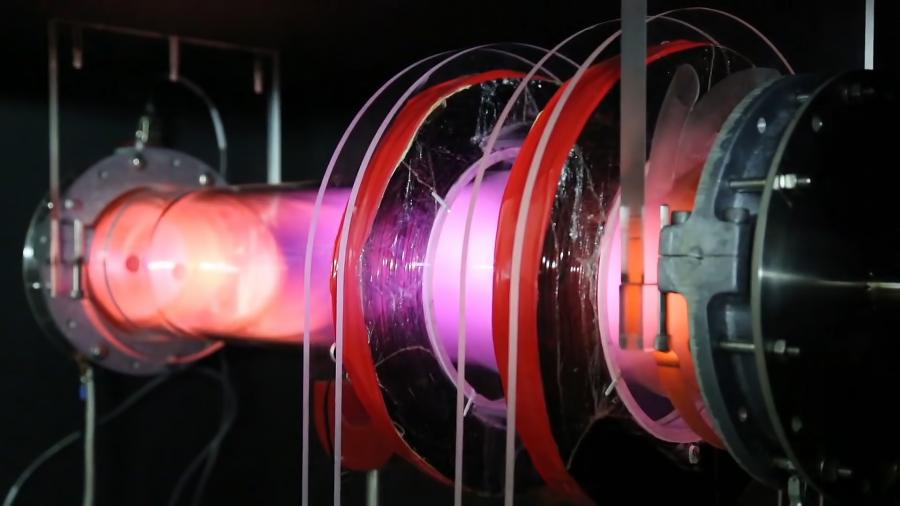
\includegraphics[width=\columnwidth]{extra/plasma2.jpg}
      \end{center}
    \end{minipage}
    \column{0.6\textwidth}
    \begin{minipage}[t]{1\textwidth}
      \begin{center}
        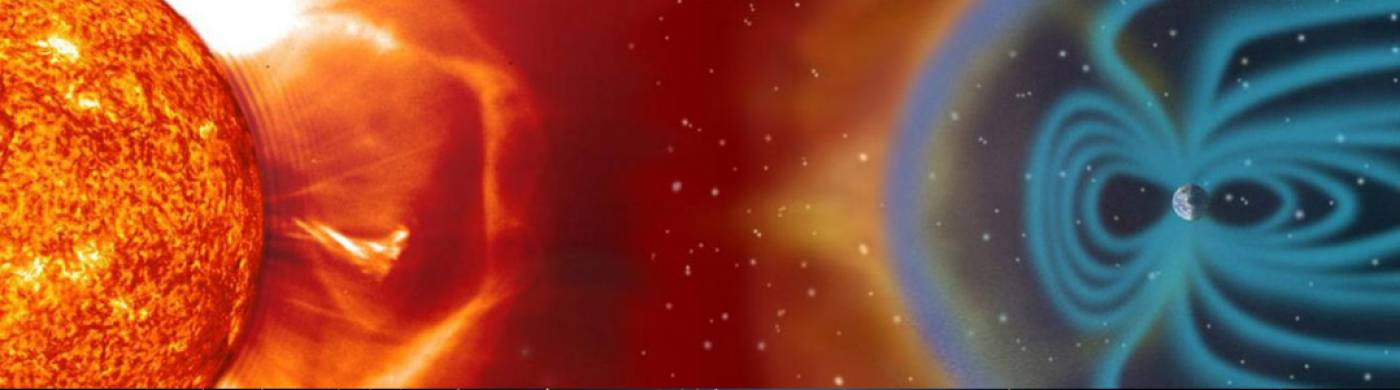
\includegraphics[width=\columnwidth]{extra/plasma1.jpg}
      \end{center}
    \end{minipage}
  \end{columns}
}
\note[itemize]{
\item DE QUÉ SIRVE LO QUE ESTUDIAMOS?
\item
\item 1) Fluido conductor que evoluciona con fuerzas Mec y EM.
\item 2) Baja colisión, baja densidad, alta velocidad alta temperatura.
\item Todo esto, arma un panorama complejo
\item
\item SIGUIENTE: MÁS COMPLEJO. TURBULENCIA.
}


\frame{\frametitle{Marco general}
  \begin{columns}
    \column{0.7\textwidth}
    \begin{minipage}[t]{1\textwidth}
Para complejizar la cuestión, en el caso del viento solar, se desarrolla
un regimen turbulento en su expansión por el medio interplanetario.
    \end{minipage}
    \column{0.3\textwidth}
    \begin{minipage}[t]{1\textwidth}
      \begin{center}
        \includegraphics[width=\columnwidth]{extra/plasma3.png}
      \end{center}
    \end{minipage}
  \end{columns}\vfill

  \begin{columns}
    \column{0.4\textwidth}
    \begin{minipage}[t]{1\textwidth}
        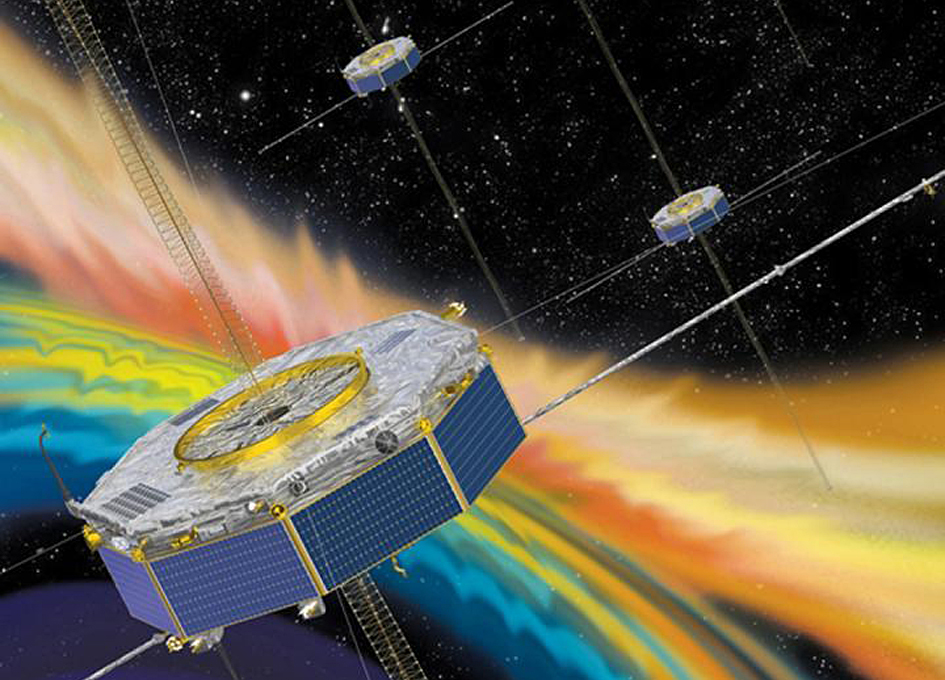
\includegraphics[width=\columnwidth]{extra/plasma4.jpg}
    \end{minipage}
    \column{0.6\textwidth}
    \begin{minipage}[t]{1\textwidth}
      \begin{flushright}
Sin embargo, hay cada vez más mediciones \emph{in situ} proporcionadas
por misiones espaciales.
      \end{flushright}
    \end{minipage}
  \end{columns}
}
\note[itemize]{
\item
\item SIGUIENTE: CÓMO SE DESCRIBE PLASMA
}


\frame{\frametitle{?`Cómo describir físicamente el plasma?}
En líneas generales, existen tres grandes enfoques posibles:
\begin{itemize}
\item Movimiento individual de las partículas.
\item Descripción cinética de una colección de partículas.
\item Descripción fluidística: magnetohidrodinámica (MHD)
\end{itemize}
La descripción MHD de un fluido describe adecuadamente la
fenomenología a grandes escalas temporales y espaciales.
}
\note[itemize]{
\item 1) $6N$ (esp fases), $N\sim 10^{15}$ en $\SI{1}{km^3}$ en medio interplanetario.
\item 2) Con funciones de distribución para cada especie, satisfaciendo ecuaciones cinéticas (como Vlasov).
\item 3) N-S con Maxwell
\item MHD se puede complejizar: dos fluidos, Hall-MHD, electron-MHD
\item Trabajaremos con MHD-1fluido con \textbf{turbulencia}
\item
\item ENTRA TURBULENCIA
}


\frame{\frametitle{Marco general}
Al igual que en el caso HD, en MHD la turbulencia introduce caos y aleatoriedad.\vfill

Algunos de los parámetros estadísticos calculables son los tiempos de
descorrelación y los espectros energéticos.\vfill

A lo largo de la presente charla, estudiaremos las correlaciones eulerianas temporales
y los espectros espacio-temporales.





}
\note[itemize]{
\item 1) Sin embargo, no de cualquier manera.
\item 1) Hay muchos parámetros estadísticos que permiten describir al plasma.
\item
\item 3) Desc lagrangiana: asociado a transferencia energética.
\item 3) Desc euleriana: predicciones limitantes.
  Está relacionada con diversos fenómenos (por ej, intermitencia).
\item 3) Las correlaciones espaciales y temporales proveen información acerca
  de la distribución espacial y temporal de la energía a lo largo de distintas escalas.
}
